\chapter{Các nón ánh sáng, đường trắc địa và chân trời Schwarzschild}

Vấn đề chân trời bắt đầu từ một sự phân biệt đã có sẵn trong thuyết tương đối hẹp. Hai sự kiện lân cận có thể được ngăn cách theo một hướng kiểu thời gian, kiểu không gian hoặc kiểu ánh sáng. Độ cong không xóa bỏ sự phân loại này. Nó khiến nón ánh sáng trở thành một đối tượng địa phương, khác nhau tại mỗi sự kiện, và khiến bản thân metric cũng trở thành một đại lượng động lực học. Một khi metric đã biết, chuyển động của một hạt rơi tự do tuân theo cùng nguyên lý thời gian riêng mô tả một hạt tương đối tính tự do trong không-thời gian phẳng.

Chúng ta sẽ dùng nguyên lý đó hai lần. Trước hết, nó phải tái tạo chuyển động Newton trong trường yếu. Sau đó, nó sẽ được áp dụng cho metric Schwarzschild, nơi ý nghĩa của thời gian, khoảng cách theo phương bán kính và vận tốc trở nên tinh tế một cách bất ngờ.

\section{Các khoảng kiểu thời gian, kiểu không gian và kiểu ánh sáng}

Trong không-thời gian phẳng, với \(c=1\), phần tử thời gian riêng là
\begin{equation}
d\tau^2=dt^2-dx^2-dy^2-dz^2.
\label{eq:l5-minkowski-proper-time}
\end{equation}
Khôi phục \(c\) là hữu ích bất cứ khi nào phép xấp xỉ phi tương đối tính có liên quan:
\begin{equation}
d\tau^2
=dt^2-\frac{dx^2+dy^2+dz^2}{c^2}.
\label{eq:l5-minkowski-c}
\end{equation}
Ký hiệu \(d\tau^2\) không bảo đảm rằng vế phải là dương. Dấu của nó dùng để phân loại độ dời:
\begin{align}
d\tau^2>0
&\quad\Longleftrightarrow\quad \text{time-like},\\
d\tau^2=0
&\quad\Longleftrightarrow\quad \text{light-like},\\
d\tau^2<0
&\quad\Longleftrightarrow\quad \text{space-like}.
\end{align}
Đối với một độ dời kiểu không gian, thuận tiện khi định nghĩa khoảng cách riêng dương
\begin{equation}
ds^2=-d\tau^2
=dx^2+dy^2+dz^2-dt^2
\qquad(c=1).
\label{eq:l5-proper-distance}
\end{equation}

Nón ánh sáng sắp xếp ba khả năng này. Chính mặt nón của nó, chứ không phải phần bên trong được lấp đầy, gồm các hướng kiểu ánh sáng. Các hướng kiểu thời gian nằm bên trong nón còn các hướng kiểu không gian nằm bên ngoài. Nửa trên và nửa dưới biểu diễn các nón ánh sáng tương lai và quá khứ.

\begin{figure}[htbp]
\centering
\includegraphics[width=0.82\textwidth]{lecture_05_figure_02.png}
\caption{Thời gian riêng, khoảng cách riêng và nón nhân quả được ghép lại trên bảng. Tia sáng nằm ngay trên bản thân nón; phần bên trong là kiểu thời gian còn phần bên ngoài là kiểu không gian.}
\lectureframe{00:05:44}
\end{figure}

\begin{figure}[htbp]
\centering
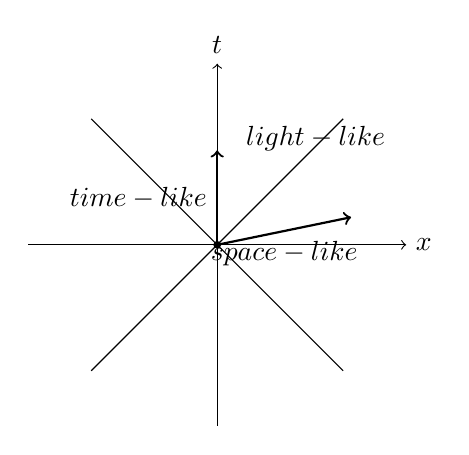
\begin{tikzpicture}[scale=1.0]
\draw[->] (0,-2.3) -- (0,2.3) node[above] {\(t\)};
\draw[->] (-2.4,0) -- (2.4,0) node[right] {\(x\)};
\draw (-1.6,1.6) -- (0,0) -- (1.6,1.6);
\draw (-1.6,-1.6) -- (0,0) -- (1.6,-1.6);
\fill (0,0) circle (1.4pt);
\draw[->,thick] (0,0) -- (0,1.2)
  node[midway,left] {\(\text{time-like}\)};
\draw[->,thick] (0,0) -- (1.7,0.35)
  node[midway,below] {\(\text{space-like}\)};
\node at (1.25,1.35) {\(\text{light-like}\)};
\end{tikzpicture}
\caption{Phân loại nhân quả trong một lát cắt không-thời gian hai chiều.}
\end{figure}

Các khoảng này được định nghĩa theo nghĩa thao tác. Thời gian riêng là số chỉ của một chiếc đồng hồ được mang dọc theo một thế giới tuyến kiểu thời gian. Khoảng cách riêng là đại lượng mà một bộ thước đo thích hợp đo giữa các sự kiện phân cách kiểu không gian. Chúng không chỉ đơn thuần là những tên gọi cho các dấu trong một dạng toàn phương.

\section{Chữ ký Lorentz và một nón tại mỗi sự kiện}

Theo quy ước tensor với đa số dấu cộng, metric phẳng có các thành phần
\begin{equation}
\eta_{\mu\nu}=\operatorname{diag}(-1,1,1,1),
\label{eq:l5-eta}
\end{equation}
và
\begin{equation}
d\tau^2=-\eta_{\mu\nu}\,dx^\mu dx^\nu.
\label{eq:l5-proper-time-eta}
\end{equation}
Ma trận được viết ra là biểu diễn của một tensor hạng hai trong một cơ sở đặc biệt đơn giản. Đặc trưng bất biến của nó là chữ ký: một hướng âm và ba hướng dương,
\begin{equation}
\operatorname{signature}(\eta)=(-,+,+,+).
\label{eq:l5-lorentz-signature}
\end{equation}
Một metric với hai dấu âm sẽ có hai hướng thời gian. Những chữ ký như vậy có thể được nghiên cứu về mặt toán học, nhưng chúng không mô tả không-thời gian được giả định ở đây.

Trong không-thời gian cong, các thành phần biến thiên:
\begin{equation}
g_{\mu\nu}=g_{\mu\nu}(x).
\label{eq:l5-position-metric}
\end{equation}
Tại mỗi sự kiện, metric vẫn phải có chữ ký Lorentz. Do đó, mỗi sự kiện có các hướng kiểu thời gian riêng, biên kiểu ánh sáng riêng và các hướng kiểu không gian riêng. Một hình vẽ theo tọa độ có thể cho thấy các nón bị nghiêng hoặc bị ép dẹt từ điểm này sang điểm khác, nhưng sự phân loại nhân quả vẫn giữ nguyên.

\begin{figure}[htbp]
\centering
\includegraphics[width=0.86\textwidth]{lecture_05_figure_03.png}
\caption{Metric phụ thuộc vị trí \(g_{\mu\nu}(x)\), các nhãn nhân quả và các phác họa của những nón ánh sáng địa phương.}
\lectureframe{00:09:41}
\end{figure}

\begin{figure}[htbp]
\centering
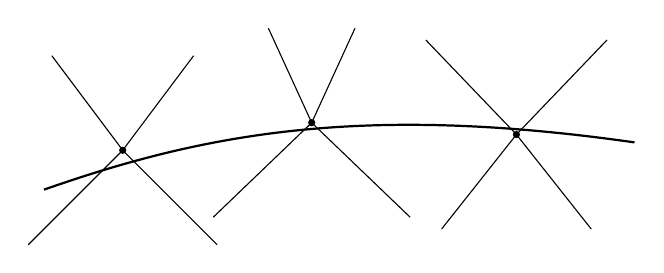
\begin{tikzpicture}[scale=1.0]
\draw[thick] (-4,-0.5) .. controls (-2,0.2) and (0,0.6) .. (3.5,0.1);
\foreach \x/\y/\a/\b in {-3/0/0.9/1.2, -0.6/0.35/0.55/1.25,
                          2.0/0.2/1.15/0.95} {
  \fill (\x,\y) circle (1.3pt);
  \draw (\x,\y) -- ++(-\a,1.2);
  \draw (\x,\y) -- ++(\a,1.2);
  \draw (\x,\y) -- ++(-\b,-1.2);
  \draw (\x,\y) -- ++(\b,-1.2);
}
\end{tikzpicture}
\caption{Các nón địa phương lân cận. Hình dạng của chúng trong tọa độ có thể thay đổi mà không làm thay đổi việc vectơ nào là kiểu thời gian, kiểu ánh sáng hay kiểu không gian.}
\end{figure}

\begin{classroomqa}
\audiencequestion{Một trị riêng âm duy nhất có chọn ra một hướng thời gian duy nhất hay không?}
\lecturerresponse{Một cơ sở làm chéo hóa ma trận được viết ra có một phương cơ sở âm, nhưng điều đó không chọn ra một quan sát viên ưu tiên hay một mũi tên vật lý duy nhất. Các phép biến đổi Lorentz trộn tọa độ thời gian với các tọa độ không gian, và mọi vectơ bên trong nón đều là kiểu thời gian. Đối tượng bất biến là nón cùng với chữ ký một âm, ba dương, chứ không phải một vectơ kiểu thời gian phân biệt nào.
\lecturetimestamp{00:12:17--00:17:24}}
\end{classroomqa}

\begin{classroomqa}
\audiencequestion{Vì sao hai hình vẽ của nón địa phương có thể có hình dạng khác nhau?}
\lecturerresponse{Tọa độ có thể làm thay đổi hình vẽ. Chẳng hạn, thay \(x\) bằng một tọa độ được co giãn lại sẽ làm thay đổi độ dốc số học gán cho một tia sáng và do đó khiến nón trông hẹp hơn hoặc rộng hơn. Các hệ tọa độ tổng quát hơn có thể làm nó nghiêng đi. Vẫn đang biểu diễn cùng một sự kiện và cùng những quan hệ nhân quả. Trong không-thời gian cong, các nón tại những sự kiện khác nhau còn thuộc về những không gian tiếp xúc khác nhau, nên việc so sánh chúng đòi hỏi metric và một quy tắc vận chuyển.
\lecturetimestamp{00:13:37--00:15:59}}
\end{classroomqa}

\section{Đường trắc địa như một bài toán biến phân}

Một hạt chuyển động tự do đi theo một đường trắc địa trong không-thời gian. Ở dạng vi phân, dùng một tham số affine \(\lambda\),
\begin{equation}
\frac{d^2x^\mu}{d\lambda^2}
+\Gamma^\mu{}_{\rho\sigma}
\frac{dx^\rho}{d\lambda}
\frac{dx^\sigma}{d\lambda}=0.
\label{eq:l5-geodesic}
\end{equation}
Liên kết cho biết vectơ tiếp tuyến phải duy trì song song với chính nó như thế nào khi hạt chuyển động.

Có một cách phát biểu thứ hai thường dễ tính toán hơn. Trong một không gian Riemann với metric \(g_{mn}\), độ dài của một đường cong là
\begin{equation}
s=\int ds
=\int\sqrt{g_{mn}\,dx^m dx^n}.
\label{eq:l5-spatial-length}
\end{equation}
Đường trắc địa làm cho độ dài này dừng dưới những biến phân nhỏ của quỹ đạo với hai đầu mút cố định. Tích phân đó đơn giản là tổng các độ dài vô cùng bé dọc theo đường cong, và phương trình Euler--Lagrange của nó là một phương trình vi phân cấp hai tương tự về hình thức với một định luật lực.

Đối với một thế giới tuyến kiểu thời gian, độ dài không gian được thay bằng thời gian riêng:
\begin{equation}
\tau
=\int\sqrt{-g_{\mu\nu}\,dx^\mu dx^\nu}.
\label{eq:l5-proper-time-functional}
\end{equation}
Một đường trắc địa kiểu thời gian làm \(\tau\) dừng và, khi so sánh với các quỹ đạo rơi tự do lân cận trước khi xuất hiện các điểm liên hợp, là cực đại cục bộ. Nhân với \(-m\) ta được tác dụng của hạt
\begin{equation}
A=-m\tau
=-m\int\sqrt{-g_{\mu\nu}\,dx^\mu dx^\nu}.
\label{eq:l5-particle-action}
\end{equation}
Do đó, cùng quỹ đạo ấy cực tiểu hóa cục bộ \(A=-m\tau\). Sự phân biệt giữa thời gian riêng dừng và dấu của tác dụng được chọn loại bỏ sự mơ hồ bề ngoài giữa cực tiểu và cực đại.

\section{Từ thời gian riêng đến một Lagrangian thông thường}

Tác dụng trong \eqref{eq:l5-particle-action} mang tính hình học, nhưng có thể được đưa về dạng quen thuộc dùng trong cơ học. Tham số hóa thế giới tuyến bằng tọa độ \(t\), chia mỗi vi phân cho \(dt\) và đưa thừa số \(dt\) còn lại ra ngoài dấu căn:
\begin{align}
A
&=-m\int\sqrt{-g_{\mu\nu}(x)\,dx^\mu dx^\nu}\\
&=-m\int
\sqrt{-g_{\mu\nu}(x)
\frac{dx^\mu}{dt}\frac{dx^\nu}{dt}}\,dt.
\label{eq:l5-action-t}
\end{align}
Đối với thành phần thời gian, ta có \(dt/dt=1\); các thành phần không gian là các vận tốc tọa độ thông thường. Vì vậy, ta có thể viết
\begin{equation}
\begin{aligned}
A&=\int L\,dt,\\
L&=-m\sqrt{-g_{\mu\nu}(x)\dot x^\mu\dot x^\nu},\\
\dot x^\mu&=\frac{dx^\mu}{dt}.
\end{aligned}
\label{eq:l5-relativistic-lagrangian}
\end{equation}

\begin{figure}[htbp]
\centering
\includegraphics[width=0.88\textwidth]{lecture_05_figure_05.png}
\caption{Tác dụng của thế giới tuyến đang được chuyển về dạng thông thường \(A=\int L\,dt\).}
\lectureframe{00:27:00}
\end{figure}

\begin{figure}[htbp]
\centering
\includegraphics[width=0.88\textwidth]{lecture_05_figure_06.png}
\caption{Một trạng thái bảng ở phần sau, với Lagrangian tương đối tính được tách riêng.}
\lectureframe{00:28:59}
\end{figure}

\begin{classroomqa}
\audiencequestion{Các chỉ số không-thời gian trong tác dụng này có nên là chữ Hy Lạp không?}
\lecturerresponse{Có. Các chỉ số Hy Lạp chạy qua thời gian và tất cả các tọa độ không gian. Chỉ số Latin có thể được dành cho các tọa độ không gian khi sự phân biệt đó hữu ích.
\lecturetimestamp{00:25:53--00:26:03}}
\end{classroomqa}

\begin{classroomqa}
\audiencequestion{Vì sao biểu thức căn bậc hai được gọi là Lagrangian?}
\lecturerresponse{Sau khi tác dụng đã được viết thành \(A=\int L\,dt\), hàm dưới dấu tích phân là Lagrangian. Đây không chỉ là một định nghĩa: biến phân hàm đó cho các phương trình Euler--Lagrange
\[
\frac{d}{dt}
\left(\frac{\partial L}{\partial\dot x^\mu}\right)
=\frac{\partial L}{\partial x^\mu},
\]
vốn tương đương với phương trình trắc địa sau khi việc tham số hóa được xử lý một cách nhất quán.
\lecturetimestamp{00:28:36--00:29:02}}
\end{classroomqa}

Đối với một hạt có khối lượng, thế giới tuyến là kiểu thời gian, nên đại lượng dưới căn bậc hai là dương. Một quỹ đạo kiểu không gian sẽ mô tả chuyển động siêu quang, chứ không phải quỹ đạo của một hạt có khối lượng thông thường. Với một metric cho trước, giờ đây có thể thu được quỹ đạo của hạt hoặc bằng cách tính các ký hiệu Christoffel và dùng \eqref{eq:l5-geodesic}, hoặc bằng cách áp dụng Euler--Lagrange cho \eqref{eq:l5-relativistic-lagrangian}. Chứng minh tính tương đương của chúng là một bài tập hữu ích; con đường qua tác dụng thường ngắn hơn.

\section{Giới hạn Newton}

Hãy xét trường hấp dẫn yếu, tĩnh bên ngoài một nguồn đối xứng cầu. Bắt đầu từ không-thời gian phẳng và cho phép hệ số của \(dt^2\) lệch nhẹ khỏi một:
\begin{equation}
d\tau^2
=\left(1+\frac{2u(\mathbf{x})}{c^2}\right)dt^2
-\frac{d\mathbf{x}^2}{c^2},
\label{eq:l5-weak-metric}
\end{equation}
trong đó \(u\) sẽ trở thành thế hấp dẫn Newton. Dạng giả định này phải được kiểm tra, chứ không chỉ đơn thuần được gọi tên.

Tác dụng có thứ nguyên của hạt là
\begin{equation}
A=-mc^2\int
\sqrt{1+\frac{2u}{c^2}
-\frac{\dot{\mathbf{x}}^{\,2}}{c^2}}\,dt.
\label{eq:l5-weak-action}
\end{equation}
Cả \(u/c^2\) lẫn \(\dot{\mathbf{x}}^{\,2}/c^2\) đều nhỏ. Giữ lại các đóng góp bậc nhất của chúng,
\begin{equation}
\sqrt{1+\epsilon}
=1+\frac{\epsilon}{2}+O(\epsilon^2),
\qquad
\epsilon=\frac{2u-\dot{\mathbf{x}}^{\,2}}{c^2},
\end{equation}
ta được
\begin{align}
L
&=-mc^2
\sqrt{1+\frac{2u-\dot{\mathbf{x}}^{\,2}}{c^2}}\\
&=-mc^2-mu+\frac{m}{2}\dot{\mathbf{x}}^{\,2}\\
&\quad+O\!\left(c^{-2}
 [u^2+u\dot{\mathbf{x}}^{\,2}+\dot{\mathbf{x}}^{\,4}]\right).
\label{eq:l5-newton-expansion}
\end{align}
Hạng năng lượng nghỉ hằng số không có ảnh hưởng lên các phương trình chuyển động. Phần còn lại là
\begin{equation}
L_{\mathrm{nr}}
=\frac{m}{2}\dot{\mathbf{x}}^{\,2}-m u(\mathbf{x}),
\label{eq:l5-newton-lagrangian}
\end{equation}
và do đó
\begin{equation}
m\ddot{\mathbf{x}}=-m\boldsymbol{\nabla}u.
\label{eq:l5-newton-equation}
\end{equation}
Khối lượng thử triệt tiêu, đúng như phải xảy ra đối với tính phổ quát của rơi tự do. Thế năng là \(m u\), còn gia tốc thì độc lập với \(m\).

Do đó, ta đã xác định được hệ thức trường yếu bậc đầu
\begin{equation}
g_{00}=1+\frac{2u}{c^2}+O(c^{-4}).
\label{eq:l5-g00-newton}
\end{equation}
Bên ngoài một khối lượng có đối xứng cầu \(M\),
\begin{equation}
u(r)=-\frac{GM}{r},
\qquad
g_{00}=1-\frac{2GM}{rc^2}+O(c^{-4}).
\label{eq:l5-g00-spherical}
\end{equation}
Điều này xác định hiệu chỉnh đầu tiên đối với thành phần thời gian. Nó vẫn chưa xác định metric đầy đủ của trường mạnh.

\section{Tọa độ cầu và phỏng đoán Schwarzschild đầu tiên}

Tọa độ cầu là tự nhiên đối với một nguồn tâm. Trong bài giảng này, \(\theta\) được đo từ mặt phẳng xích đạo thay vì từ cực, nên phần tử độ dài góc là
\begin{equation}
d\Omega^2=d\theta^2+\cos^2\theta\,d\phi^2.
\label{eq:l5-angular-metric}
\end{equation}
Với quy ước này,
\begin{equation}
d\mathbf{x}^2=dr^2+r^2d\Omega^2.
\label{eq:l5-flat-spherical}
\end{equation}
Không có gì về mặt vật lý phụ thuộc vào việc chọn \(\theta\) kiểu vĩ độ này; nếu dùng góc cực thông dụng hơn thì \(\cos^2\theta\) sẽ được thay bằng
\(\sin^2\theta\).

Thay hệ số thời gian Newton vào mà vẫn giữ metric không gian phẳng cho ta phỏng đoán đầu tiên
\begin{equation}
\begin{aligned}
d\tau^2
&=\left(1-\frac{r_s}{r}\right)dt^2
-\frac{1}{c^2}\left(dr^2+r^2d\Omega^2\right),\\
r_s&=\frac{2GM}{c^2}.
\end{aligned}
\label{eq:l5-naive-schwarzschild}
\end{equation}
Đây không thể là nghiệm chính xác. Với \(r<r_s\), hệ số của \(dt^2\) đổi dấu trong khi mọi hệ số không gian vẫn âm theo quy ước thời gian riêng. Khi đó metric sẽ mất chữ ký với một chiều thời gian và ba chiều không gian của nó.

Các phương trình trường chân không cung cấp hệ số hướng kính cần thiết:
\begin{equation}
\boxed{
d\tau^2
=\left(1-\frac{r_s}{r}\right)dt^2
-\frac{dr^2}{c^2\left(1-r_s/r\right)}
-\frac{r^2}{c^2}d\Omega^2.
}
\label{eq:l5-schwarzschild}
\end{equation}
Đây là metric Schwarzschild bên ngoài. Khi \(r\) đi qua \(r_s\), các hệ số của \(t\) và \(r\) cùng đổi dấu, nhờ đó bảo toàn chữ ký Lorentz. Trong tọa độ Schwarzschild, tọa độ hướng kính trở thành dạng thời gian ở phía trong và tọa độ \(t\) trở thành dạng không gian. Sự hoán đổi này báo hiệu sự thất bại của biểu đồ tọa độ tại chân trời, chứ không phải sự thất bại cục bộ của hình học không-thời gian.

\begin{classroomqa}
\audiencequestion{Một vật rơi mất bao lâu để đi qua chân trời?}
\lecturerresponse{Nếu đo bằng tọa độ Schwarzschild \(t\) mà một quan sát viên ở xa dùng, sự băng qua bị đẩy ra tới thời gian vô hạn. Nếu đo bằng thời gian riêng trên đồng hồ của vật rơi, nó diễn ra trong thời gian hữu hạn. Sự phân biệt giữa hai đồng hồ này là câu đố cốt lõi về chân trời.
\lecturetimestamp{00:54:45--00:55:35}}
\end{classroomqa}

\begin{classroomqa}
\audiencequestion{Vì sao phải thay đổi hệ số hướng kính chứ không phải phần nào khác của metric?}
\lecturerresponse{Metric phải giữ chữ ký Lorentz, đối xứng cầu phân biệt phương hướng kính với mặt cầu góc, và các phương trình trường chân không xác định chính xác thừa số nghịch đảo. Chỉ riêng yêu cầu về chữ ký cho ta biết nên tìm ở đâu; các phương trình Einstein cho kết quả chính xác.
\lecturetimestamp{00:55:35--00:56:01}}
\end{classroomqa}

Đối với Trái Đất, \(r_s\) chỉ cỡ một xentimét, nằm sâu bên trong khối vật chất. Metric chân không bên ngoài không còn đúng ở đó, nên Trái Đất không có chân trời Schwarzschild. Một nghiệm nội phải thay thế nó bên trong vật chất và ghép khớp với nó tại bề mặt.

\begin{classroomqa}
\audiencequestion{Nếu \(t\) và \(r\) hoán đổi vai trò tọa độ, thì một đồng hồ bình thường sẽ ra sao?}
\lecturerresponse{Đồng hồ vẫn tiếp tục đo thời gian riêng dọc theo một đường thế giới dạng thời gian. Nó không biết rằng một tọa độ đã chọn trở nên bất tiện. Một hệ tọa độ rơi tự do chính quy cho thấy hình học cục bộ trơn tru và sự truyền ánh sáng cục bộ hoàn toàn bình thường qua chân trời.
\lecturetimestamp{00:56:35--00:57:50}}
\end{classroomqa}

\subsection{Vì sao hiệu chỉnh hướng kính đã không xuất hiện trong phương trình Newton}

Metric chính xác làm thay đổi hệ số hướng kính ngay từ bậc nhất theo thế:
\begin{equation}
\frac{1}{1-r_s/r}
=1+\frac{r_s}{r}
+O\!\left(\frac{r_s^2}{r^2}\right)
=1-\frac{2u}{c^2}+O(c^{-4}).
\label{eq:l5-radial-expansion}
\end{equation}
Vì sao có thể chính đáng bỏ qua sự thay đổi đó trong phép suy dẫn Newton? Trong phiếm hàm tác dụng của hạt, nó nhân với \(\dot r^2/c^2\). Vì vậy hiệu chỉnh bậc nhất của nó tỉ lệ với
\begin{equation}
\frac{u\,\dot r^2}{c^4},
\end{equation}
là bậc cao hơn mức được giữ lại trong
\eqref{eq:l5-newton-expansion}. Hiệu chỉnh hướng kính là không đáng kể đối với phép kiểm tra Newton ở giới hạn chuyển động chậm, nhưng lại trở nên quyết định đối với chuyển động tương đối tính và ở gần chân trời. Đây là một lời nhắc hữu ích: một hạng tử quá nhỏ đối với một phép gần đúng có thể chi phối hiện tượng đang quan tâm trong một phép gần đúng khác.

\section{Sự rơi hướng kính theo thời gian Schwarzschild}

Đặt \(c=1\) và trước hết xét chuyển động hướng kính. Các quỹ đạo tròn cũng quan trọng, nhưng chúng đòi hỏi các hạng góc nên được hoãn lại. Chuyển động hướng kính không hẳn là một quỹ đạo mà đúng hơn là một cú lao thẳng về nguồn, và nó bộc lộ hành vi của chân trời với lượng đại số ít nhất.

\begin{classroomqa}
\audiencequestion{Thời gian của ai xuất hiện trong vận tốc hướng kính?}
\lecturerresponse{Dấu chấm bên dưới có nghĩa là đạo hàm theo thời gian tọa độ Schwarzschild \(t\), tức thời gian được chuẩn hóa theo quan sát viên tĩnh ở xa. Đồng hồ đeo tay của quan sát viên rơi đo thời gian riêng \(\tau\). Lẫn lộn hai đại lượng này sẽ biến một phát biểu tọa độ thành một phát biểu cục bộ sai.
\lecturetimestamp{01:04:03--01:04:47}}
\end{classroomqa}

Với \(d\Omega=0\), hãy định nghĩa
\begin{equation}
a(r)=1-\frac{r_s}{r}.
\label{eq:l5-a-def}
\end{equation}
Metric hướng kính và Lagrangian là
\begin{align}
d\tau^2&=a\,dt^2-\frac{dr^2}{a},\\
L&=-m\sqrt{a-\frac{\dot r^2}{a}},
\qquad
\dot r=\frac{dr}{dt}.
\label{eq:l5-radial-lagrangian}
\end{align}
Vì \(L\) không phụ thuộc tường minh vào \(t\), Hamiltonian của nó được bảo toàn.
Xung lượng hướng kính là
\begin{equation}
p_r=\frac{\partial L}{\partial\dot r}
=\frac{m\dot r}{a\sqrt{a-\dot r^2/a}},
\label{eq:l5-radial-momentum}
\end{equation}
và
\begin{align}
H
&=p_r\dot r-L\\
&=\frac{ma}{\sqrt{a-\dot r^2/a}}
=E.
\label{eq:l5-radial-energy}
\end{align}
Giải theo vận tốc tọa độ, ta được
\begin{equation}
\boxed{
\dot r^2
=a^2\left(1-\frac{m^2}{E^2}a\right).
}
\label{eq:l5-radial-velocity}
\end{equation}
Phép tính trên bảng thử qua một số dạng đại số trung gian; biểu thức đóng khung là kết quả nhất quán.

Khi \(r\) tiến tới \(r_s\), \(a(r)\) tiến về không còn thừa số trong ngoặc tiến về một. Do đó
\begin{equation}
\frac{dr}{dt}
\sim -\left(1-\frac{r_s}{r}\right)
\longrightarrow 0
\qquad(r\longrightarrow r_s^+)
\label{eq:l5-infall-freeze}
\end{equation}
đối với một hạt đi vào trong. Theo thời gian Schwarzschild, hạt dường như chậm lại và bị đóng băng ngay bên ngoài chân trời.

\begin{classroomqa}
\audiencequestion{Giá trị giảm dần của \(dr/dt\) có nghĩa là hấp dẫn đã trở nên đẩy ra sao?}
\lecturerresponse{Không. Hạt không bị đẩy ra ngoài theo nghĩa cục bộ. Tọa độ \(t\) ngày càng không thích hợp để mô tả sự băng qua, nên độ tiến hướng kính trên mỗi đơn vị \(t\) tiến về không. Gia tốc riêng dọc theo đường thế giới rơi tự do vẫn bằng không, và chân trời được chạm tới trong thời gian riêng hữu hạn.
\lecturetimestamp{01:14:18--01:16:38}}
\end{classroomqa}

Thật vậy, gần chân trời
\begin{equation}
\frac{dt}{dr}
\sim-\frac{1}{1-r_s/r}
=-\frac{r}{r-r_s}.
\end{equation}
Tích phân của nó phân kỳ lôgarit. Điều này chứng minh phát biểu về thời gian Schwarzschild vô hạn mà không hàm ý số chỉ vô hạn trên đồng hồ của vật rơi.

\section{Các tia sáng hướng kính}

Ánh sáng cho phiên bản ngắn gọn nhất của cùng phép tính đó. Đối với một tia null hướng kính,
\begin{equation}
d\tau^2
=a\,dt^2-\frac{dr^2}{a}=0.
\end{equation}
Do đó
\begin{equation}
\boxed{
\frac{dr}{dt}
=\pm a(r)
=\pm\left(1-\frac{r_s}{r}\right).
}
\label{eq:l5-radial-light}
\end{equation}
Dấu cộng mô tả một tia đi ra ngoài và dấu trừ mô tả một tia đi vào trong. Cả hai vận tốc tọa độ đều tiến về không tại chân trời.

\begin{classroomqa}
\audiencequestion{Công thức cho tốc độ nào ở xa nguồn?}
\lecturerresponse{Khi \(r\) tiến tới vô cực, \(a(r)\) tiến tới một, nên \(dr/dt\) tiến tới \(\pm1\), hay \(\pm c\) khi khôi phục đơn vị.
\lecturetimestamp{01:21:01--01:21:29}}
\end{classroomqa}

Thuyết tương đối rộng thường là như vậy: các nguyên lý gói gọn trong vài dòng, trong khi tọa độ và phép tính trở nên phức tạp. Phương trình
\eqref{eq:l5-radial-light}
rất đơn giản, nhưng việc diễn giải việc nó tiến về không gần
\(r_s\)
đòi hỏi sự cẩn trọng. Đó là một vận tốc tọa độ, không phải vận tốc do một quan sát viên quán tính cục bộ đo được.

\section{Những gì một quan sát viên ở xa nhìn thấy}

\begin{classroomqa}
\audiencequestion{Ánh sáng phát ra gần chân trời có thể thoát ra không, và đó có phải là bức xạ Hawking không?}
\lecturerresponse{Một tia cổ điển đi ra ngoài được phát ra ngay bên ngoài chân trời có thể chuyển động ra ngoài, nhưng vận tốc tọa độ Schwarzschild của nó khởi đầu cực nhỏ và tín hiệu chỉ tới vô cực sau một độ trễ và dịch đỏ rất mạnh. Một tia nằm trên chân trời thì vẫn ở trên chân trời trong các tọa độ này; một tia ở phía trong thì không thể thoát ra. Bức xạ Hawking là một hiệu ứng trường lượng tử gắn với hình học bên ngoài, không phải một tia sáng cổ điển leo ra từ bên trong, và nó không được suy ra bằng phép tính hiện tại.
\lecturetimestamp{01:22:08--01:24:28}}
\end{classroomqa}

\begin{classroomqa}
\audiencequestion{Nếu một photon trông gần như đứng yên, liệu nó có bắt đầu trông như có khối lượng không?}
\lecturerresponse{Không. Một quan sát viên cục bộ rơi tự do luôn đo photon chuyển động với \(c\). Chỉ có tỉ số tọa độ \(dr/dt\) tiến về không. Khối lượng, tính chất null và tốc độ ánh sáng cục bộ không bị thay đổi bởi một biểu đồ tọa độ tồi.
\lecturetimestamp{01:24:31--01:25:26}}
\end{classroomqa}

Biểu thức Schwarzschild dùng ở đây là một nghiệm chân không bên ngoài. Một ngôi sao, hành tinh hay đám mây đang suy sụp có metric bên trong khác, và metric đó phải được khớp với nghiệm này. Nếu bề mặt vật chất vẫn nằm ngoài \(r_s\), như bề mặt Trái Đất nằm ngoài đó một khoảng cực lớn, thì chân trời tọa độ của nghiệm ngoài nằm ngoài miền mà công thức chân không có thể được kéo dài xuyên qua vật chất. Nếu vật thể suy sụp vào bên trong bán kính Schwarzschild của nó, chân trời trở thành một phần của không-thời gian vật lý.

\begin{classroomqa}
\audiencequestion{Nếu một quan sát viên bên ngoài không bao giờ thấy vật chất băng qua, thì làm sao một hố đen có thể hình thành hoặc lớn lên?}
\lecturerresponse{Tiền đề ấy dùng thời gian Schwarzschild như thể nó là một đồng hồ vật lý toàn cục tại chân trời. Kết luận rằng vì thế một hố đen không bao giờ có thể lớn lên nghe có vẻ hợp lý nhưng là sai. Một câu trả lời đầy đủ đòi hỏi các tọa độ chính quy băng qua chân trời và hình học nhân quả toàn cục của sự suy sụp; lời giải quyết đó được hoãn lại đến phần kế tiếp của khóa học.
\lecturetimestamp{01:27:57--01:29:36}}
\end{classroomqa}

\begin{classroomqa}
\audiencequestion{Một súng radar sẽ cho biết gì về một chiếc xe đang rơi về phía chân trời?}
\lecturerresponse{Vận tốc tọa độ lúc đầu tăng khi xe rơi xuống, rồi bẻ ngoặt và giảm dần về không. Các xung radar gửi đi muộn hơn vẫn có thể bắt kịp xe ở ngoài chân trời, nhưng hành trình khứ hồi kéo dài dần. Tín hiệu phản hồi bị dịch đỏ ngày càng mạnh, và hình ảnh dường như chậm lại và bị nén gần \(r_s\). Đây không phải là một bức tranh cục bộ đáng tin về điều mà người lái trải nghiệm; người đó băng qua trong thời gian riêng hữu hạn.
\lecturetimestamp{01:29:39--01:32:14}}
\end{classroomqa}

\begin{classroomqa}
\audiencequestion{Tốc độ ánh sáng có phải chỉ không đổi trong thuyết tương đối hẹp không?}
\lecturerresponse{Nó cũng không đổi trong mọi hệ quy chiếu quán tính địa phương của thuyết tương đối rộng. Một quan sát viên đang rơi, dùng các đồng hồ và thước mét địa phương, đo một photon ở gần có tốc độ \(c\). Những tốc độ tọa độ như \(dr/dt\) có thể thay đổi vì \(r\) và \(t\) không phải là các số đọc của một phòng thí nghiệm quán tính địa phương duy nhất trên toàn bộ không-thời gian.
\lecturetimestamp{01:32:20--01:34:20}}
\end{classroomqa}

\section{Những câu hỏi vượt ra ngoài phép tính Schwarzschild}

\begin{classroomqa}
\audiencequestion{Thống nhất hấp dẫn với các lực khác có thể có nghĩa là gì?}
\lecturerresponse{Một khả năng hình học là mở rộng không-thời gian bằng các chiều compact bổ sung. Khi đó, các thành phần của một metric nhiều chiều hơn có thể xuất hiện trong bốn chiều dưới dạng các trường chuẩn và các trường vô hướng, còn động lượng theo một chiều phụ thêm có thể xuất hiện như một điện tích. Đây là một gợi ý về mặt cấu trúc gắn với các ý tưởng Kaluza--Klein, chứ không phải một sự thống nhất đã hoàn chỉnh trong bài giảng hiện tại.
\lecturetimestamp{01:34:22--01:36:08}}
\end{classroomqa}

\begin{classroomqa}
\audiencequestion{Liệu các miền hay các vũ trụ khác nhau có thể có các chữ ký metric khác nhau không?}
\lecturerresponse{Thuyết tương đối rộng cổ điển thông thường ấn định một chữ ký Lorentzian không suy biến. Muốn thay đổi nó, metric sẽ phải đi qua một cấu hình suy biến, nơi mô tả cổ điển tiêu chuẩn không còn hiệu lực. Hấp dẫn lượng tử có thể buộc ta phải dùng một ngôn ngữ rộng hơn, nhưng ở đây không có lý thuyết nào đã được xác lập dự đoán những miền vật lý có sự thay đổi chữ ký.
\lecturetimestamp{01:36:08--01:38:08}}
\end{classroomqa}

\begin{classroomqa}
\audiencequestion{Schwarzschild đã tìm ra nghiệm này như thế nào khi đang phục vụ trong Chiến tranh thế giới thứ nhất?}
\lecturerresponse{Điểm được nêu trên lớp mang tính con người không kém gì tính lịch sử: Schwarzschild là một nhà thiên văn học và một nhà toán học hết sức xuất sắc, và việc nghiền ngẫm các phương trình mới của Einstein đã đem lại cho ông một nơi nương náu về trí tuệ giữa lúc phục vụ thời chiến.
\lecturetimestamp{01:38:11--01:39:02}}
\end{classroomqa}

Bài học cốt lõi giờ đây đã đủ rõ để mang sang phần tiếp theo. Metric quyết định cả các nón nhân quả lẫn chuyển động tự do. Thành phần thời gian của nó trong trường yếu chứa thế Newton, còn dạng Schwarzschild chính xác của nó xác định một chân trời tọa độ tại \(r=r_s\). Thời gian Schwarzschild kéo dài việc đi qua ấy ra tới vô hạn; còn thời gian riêng của quan sát viên đang rơi thì không. Bài toán tiếp theo là giải quyết sự tương phản đó trên bình diện toàn cục, và giải thích cách một lỗ đen hình thành bất chấp hình ảnh ở xa bị đóng băng.